% This file was created with tikzplotlib v0.10.1.post9.
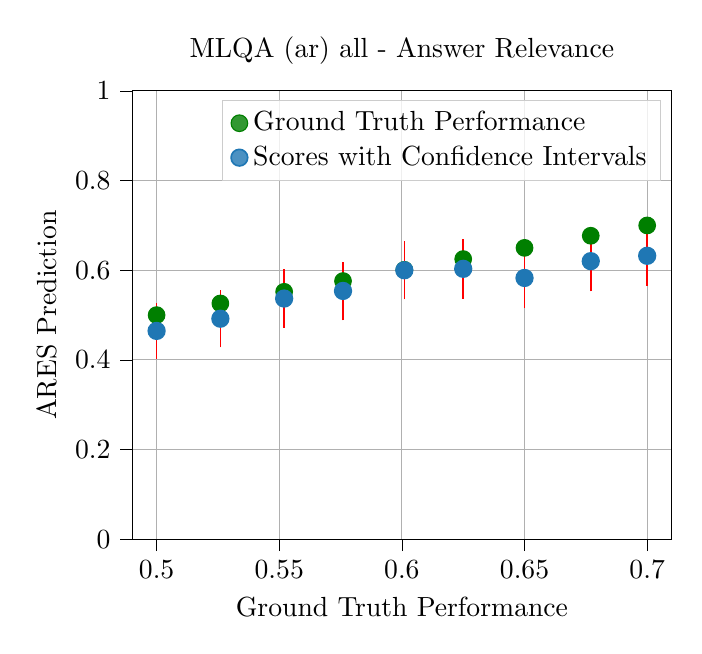
\begin{tikzpicture}

\definecolor{darkgrey176}{RGB}{176,176,176}
\definecolor{green01270}{RGB}{0,127,0}
\definecolor{lightgrey204}{RGB}{204,204,204}
\definecolor{steelblue31119180}{RGB}{31,119,180}

\begin{axis}[
legend cell align={left},
legend style={
  fill opacity=0.8,
  draw opacity=1,
  text opacity=1,
  draw=lightgrey204,
  mark options={mark size=3}
},
tick align=outside,
tick pos=left,
title={MLQA (ar) all - Answer Relevance},
x grid style={darkgrey176},
xlabel={Ground Truth Performance},
xmajorgrids,
xmin=0.49, xmax=0.71,
xtick style={color=black},
y grid style={darkgrey176},
ylabel={ARES Prediction},
ymajorgrids,
ymin=0, ymax=1,
ytick style={color=black}
]
\addplot [draw=green01270, fill=green01270, mark size=3pt, mark=*, only marks]
table{%
x  y
0.5 0.5
0.526 0.526
0.552 0.552
0.576 0.576
0.601 0.601
0.625 0.625
0.65 0.65
0.677 0.677
0.7 0.7
};
\addlegendentry{Ground Truth Performance}
\path [draw=red, semithick]
(axis cs:0.5,0.401)
--(axis cs:0.5,0.528);

\path [draw=red, semithick]
(axis cs:0.526,0.428)
--(axis cs:0.526,0.556);

\path [draw=red, semithick]
(axis cs:0.552,0.472)
--(axis cs:0.552,0.602);

\path [draw=red, semithick]
(axis cs:0.576,0.488)
--(axis cs:0.576,0.619);

\path [draw=red, semithick]
(axis cs:0.601,0.535)
--(axis cs:0.601,0.665);

\path [draw=red, semithick]
(axis cs:0.625,0.537)
--(axis cs:0.625,0.669);

\path [draw=red, semithick]
(axis cs:0.65,0.515)
--(axis cs:0.65,0.65);

\path [draw=red, semithick]
(axis cs:0.677,0.553)
--(axis cs:0.677,0.687);

\path [draw=red, semithick]
(axis cs:0.7,0.565)
--(axis cs:0.7,0.7);

\addplot [semithick, steelblue31119180, mark=*, mark size=3, mark options={solid}, only marks]
table {%
0.5 0.464725274725275
0.526 0.492023121387283
0.552 0.536969696969697
0.576 0.553924050632912
0.601 0.60006600660066
0.625 0.603230240549828
0.65 0.582857142857143
0.677 0.620297397769517
0.7 0.632307692307692
};
\addlegendentry{Scores with Confidence Intervals}
\end{axis}

\end{tikzpicture}
